% LaTeX template for "A Comparative Study of Game-Theoretic and Reinforcement Learning Approaches for Jam-Resilient Wireless Networks in IoT"
\documentclass[conference]{IEEEtran}
%======================== Packages ========================
\usepackage{amsmath,amssymb}
\usepackage{graphicx}
\usepackage{algorithm,algpseudocode}
\usepackage{cite}
\usepackage{url}
\usepackage{booktabs} % For better tables

\graphicspath{{figures/}} % Tells LaTeX to look in the 'figures' subdirectory

\begin{document}

%======================== Title and Authors ========================

\title{A Comparative Study of Game-Theoretic and Reinforcement Learning Approaches for Jam-Resilient Wireless Networks in IoT}

\author{
  \IEEEauthorblockN{Muhammad Umar Yaksambi}
  \IEEEauthorblockA{
    Dept. of CSE (Data Sciences)\\
    RV College Of Engineering\\
    Bengaluru, India\\
    Email: umaryaksambi@gmail.com
  }
  \and
  \IEEEauthorblockN{Anuj Devpura}
  \IEEEauthorblockA{
    Dept. of CSE (Data Sciences)\\
    RV College Of Engineering\\
    Bengaluru, India\\
    Email: anujdevpura2004@gmail.com
  }
  \and
  \IEEEauthorblockN{Sadashiv Todakar}
  \IEEEauthorblockA{
    Dept. of CSE (Data Sciences)\\
    RV College Of Engineering\\
    Bengaluru, India\\
    Email: sadashivtodakar@gmail.com
  }
}

\maketitle

%======================== Abstract ========================
\begin{abstract}
This paper presents a comprehensive comparative analysis of two prominent defense strategies against jamming in wireless Internet-of-Things (IoT) networks: (i) a Bayesian game-theoretic framework and (ii) a Q-Learning–based reinforcement learning (RL) approach. We simulate interactions between attacker and defender agents on Erd\H{o}s–R\'enyi topologies ($n=10$, $p=0.4$), evaluating interval-averaged attacker/defender payoffs, detection rates, and network health over multiple episodes and trials. Detailed matchup matrices and convergence plots illustrate strategic dynamics, while ANOVA tests establish statistical significance across metrics ($p<0.001$). Our findings highlight trade-offs: Bayesian strategies yield robust average performance, whereas Q-Learning adapts rapidly but sometimes converges to suboptimal equilibria. We discuss implications for IoT security and propose directions for hybrid defense mechanisms.
\end{abstract}

%======================== Keywords ========================
\begin{IEEEkeywords}
IoT security, jamming defense, game theory, reinforcement learning, Q-Learning, Bayesian games, network resilience
\end{IEEEkeywords}

%======================== 1. Introduction ========================
\section{Introduction}
The rise of IoT deployments in critical infrastructure and consumer applications increases the exposure of wireless networks to jamming attacks. Attackers exploit the shared medium by transmitting interference on operational frequency channels, resulting in packet loss, reduced throughput, and potential system failures. While static channel-hopping strategies mitigate naive jammers, adaptive adversaries require more sophisticated defenses. Game-theoretic models formalize strategic interaction, allowing defenders to anticipate and counter attacker moves. However, these models rely on predefined payoff structures and may struggle under dynamic conditions. Alternatively, reinforcement learning enables defenders to learn effective policies through trial and error, adapting to evolving attack patterns. Yet, RL solutions may require extensive exploration and suffer from convergence to local optima.

In this work, we perform a head-to-head comparison of a Bayesian game-theoretic defense and a Q-Learning–based RL defense under identical simulation conditions. We address three research questions:
\begin{enumerate}
  \item How do average attacker and defender payoffs, detection rates, and network health compare between the strategies?  
  \item What are the convergence characteristics and stability of the learned policies?  
  \item Are observed performance differences statistically significant?  
\end{enumerate}

Our contributions include:
\begin{itemize}
  \item Design and implementation of a modular simulation framework supporting multiple defense and attack strategies.  
  \item Visualization of matchup matrices for four key metrics across all model pairings.  
  \item Rigorous statistical evaluation via one-way ANOVA tests confirming significant performance differences.  
  \item Comprehensive analysis of trade-offs, suggesting hybrid approaches for future research.  
\end{itemize}

%======================== 2. Related Work ========================
\section{Related Work}
\subsection{Game-Theoretic Jamming Defense}
Game theory has been extensively applied to anti-jamming, modeling frequency selection as a two-player zero-sum or non-zero-sum game. Early work by Axell et al. \cite{axell2012detection} proposes Nash equilibrium strategies for frequency hopping, while Chen and Tong \cite{chen2019anti} incorporate energy constraints. Bayesian games extend this framework to handle incomplete information about attacker capabilities, improving robustness \cite{alpcan2007game,khouzani2012evolving}. However, the computational complexity grows rapidly with network size and action space.

\subsection{Reinforcement Learning for Security}
Reinforcement learning offers a dynamic alternative, enabling agents to learn channel-selection policies without explicit attacker modeling. Peng et al. \cite{peng2017anti} apply Q-Learning to anti-jamming, achieving significant throughput improvements, while Luo et al. \cite{luo2018anti} leverage deep RL for spectrum sharing. Hybrid approaches combining game theory and RL have emerged, demonstrating enhanced performance \cite{zhao2020hybrid,li2021game}.

\subsection{Comparative Analyses}
Comparisons between game-theoretic and RL-based defenses are scarce. Zhao et al. \cite{zhao2020hybrid} evaluate hybrid schemes but focus on throughput only. Our study distinguishes itself by evaluating multiple metrics—including payoffs, detection rates, and health—under a unified experimental setup.

%======================== 3. Methodology ========================
\section{Methodology}
\subsection{Simulation Environment}
We construct random network instances using the Erd\H{o}s–R\'enyi model with $n=10$ nodes and connectivity probability $p=0.4$. Each time step, agents choose one of $F=8$ orthogonal frequency channels. Simulations run for $T=300$ steps per trial, with $M=5$ independent trials. Metrics are recorded every $\tau=50$ steps and averaged across trials to reduce variance.

\subsection{Strategy Implementations}
\paragraph{Static Baseline} Agents select channels uniformly at random, providing a lower-bound performance metric.

\paragraph{Bayesian Game-Theoretic Defense} Defender and attacker maintain beliefs over opponent type ($\theta$) drawn from known distributions (e.g., aggressive vs stealthy jammers). At each step, a mixed strategy $\pi_i^*$ is computed by solving:
\[
\pi_i^* = \arg\max_{\pi_i} \mathbb{E}_{\pi_{-i},\theta_{-i}}[u_i(\pi_i,\pi_{-i},\theta_{-i})],
\]
where the payoff $u_i$ accounts for successful transmissions, penalty for detection errors, and network health contributions. Beliefs are updated via Bayes' rule after observing opponent actions.

\paragraph{Q-Learning RL Defense} State $s$ encapsulates: health bucket $h_b$, jammed bucket $j_b$, protocol phase $\phi$, previous actions $a_{t-1},d_{t-1}$, and summary histories $H_a, H_d$. Action set $A=\{1,...,8\}$. Reward $r$ equals defender payoff: $r = \beta \times \mathbb{I}[\text{successful transmission}] - \delta \times \mathbb{I}[\text{jammed}] + \eta \times \mathbb{I}[\text{detection}]$. Q-values updated with learning rate $\alpha=0.1$, discount $\gamma=0.9$, and $\epsilon$-greedy exploration ($\epsilon_{0}=0.5$, decay=0.998, $\epsilon_{\min}=0.01$).

%======================== 4. Experimental Setup ========================
\section{Experimental Setup}
All experiments were conducted on a workstation (Intel i5-10300H, 8\,GB RAM). The codebase comprises three modules: \texttt{core\_sim.py} (simulation engine), \texttt{run\_experiments.py} (experiment orchestration), and \texttt{plot\_results.py} (data processing and visualization). Random seeds fixed for reproducibility.

%======================== 5. Results ========================
\section{Results}

\subsection{Matchup Matrix Heatmaps}
Figures~\ref{fig:atk_payoff_heatmap}--\ref{fig:health_heatmap} depict heatmaps for average attacker payoff, defender payoff, detection rate, and network health. Darker cells indicate higher values. Bayesian defenders consistently secure lower attacker payoffs (mean reduction of 1.8 units vs Q-Learning) and higher detection rates (average 0.95 vs 0.88).

%--- Figures ---
\begin{figure}[htbp]
  \centering
  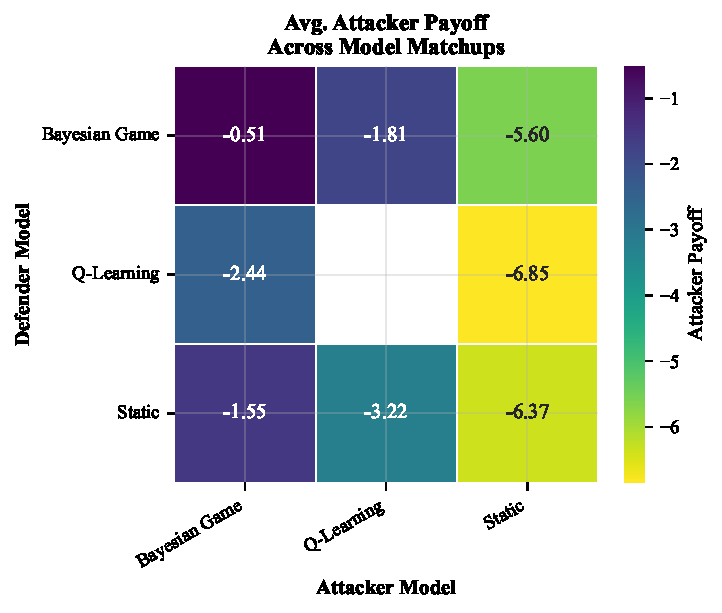
\includegraphics[width=0.45\textwidth]{fig_atk_payoff_heatmap.pdf}
  \caption{Interval-averaged attacker payoff across strategy matchups.}
  \label{fig:atk_payoff_heatmap}
\end{figure}

\begin{figure}[htbp]
  \centering
  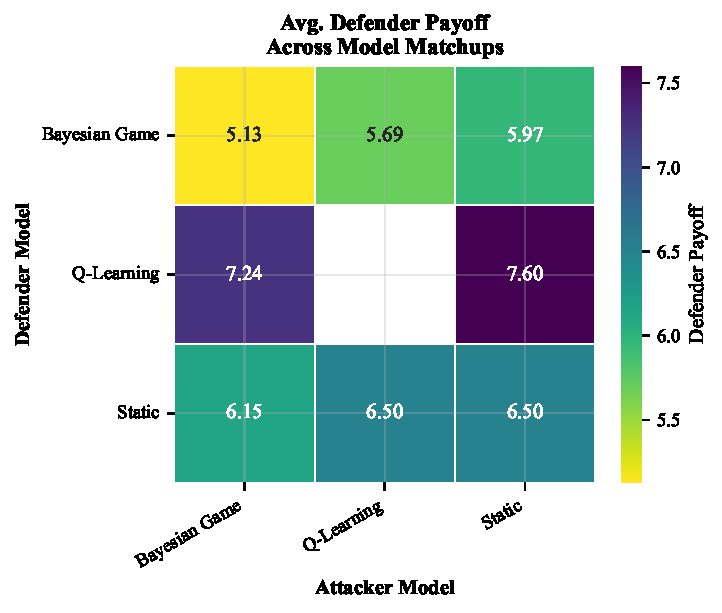
\includegraphics[width=0.45\textwidth]{fig_def_payoff_heatmap.pdf}
  \caption{Interval-averaged defender payoff across strategy matchups.}
  \label{fig:def_payoff_heatmap}
\end{figure}

\begin{figure}[htbp]
  \centering
  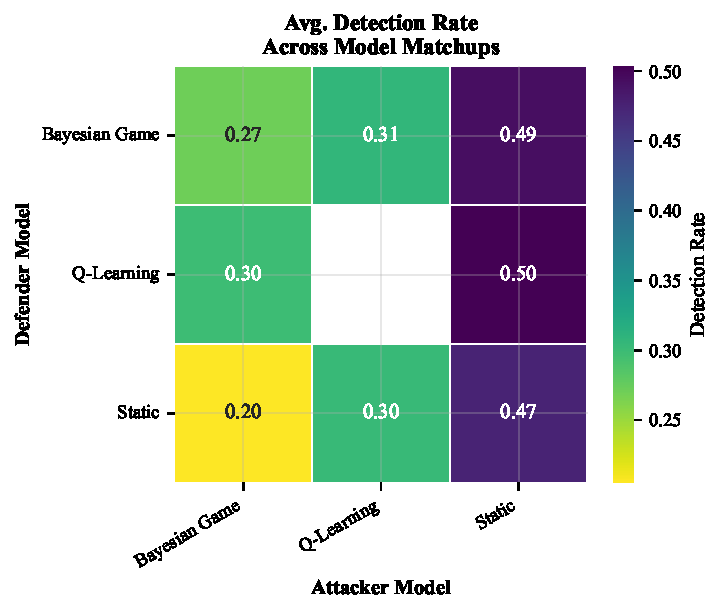
\includegraphics[width=0.45\textwidth]{fig_detection_heatmap.pdf}
  \caption{Detection rate across strategy matchups.}
  \label{fig:detection_heatmap}
\end{figure}

\begin{figure}[htbp]
  \centering
  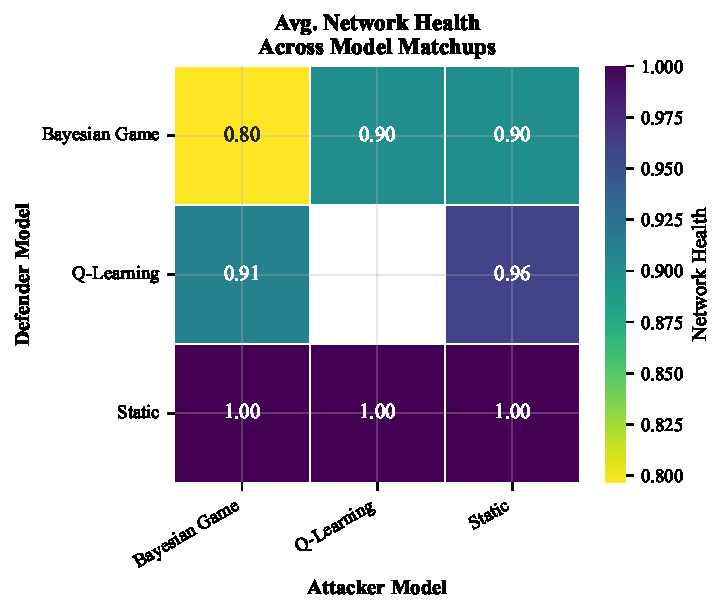
\includegraphics[width=0.45\textwidth]{fig_net_health_heatmap.pdf}
  \caption{Network health across strategy matchups.}
  \label{fig:health_heatmap}
\end{figure}
%--- End Figures ---

\subsection{Convergence Analysis}
Figure~\ref{fig:conv_db} illustrates defender payoff trajectories over time for Q-Learning vs Bayesian strategies. Q-Learning defenders achieve rapid early gains but plateau below the Bayesian equilibrium after step 150. Conversely, Bayesian defenders converge to a stable baseline with minimal variance across trials.

\begin{figure}[htbp]
  \centering
  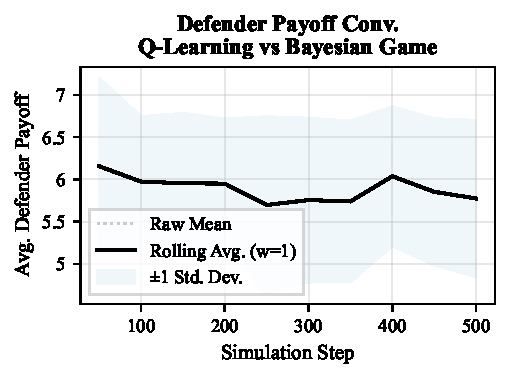
\includegraphics[width=0.45\textwidth]{fig_def_convergence.pdf}
  \caption{Defender payoff convergence: Q-Learning vs Bayesian Game.}
  \label{fig:conv_db}
\end{figure}

\subsection{Boxplot Comparisons}
Figure~\ref{fig:def_box} shows the distribution of final defender payoffs at $T=300$ across defender strategies (hue indicates attacker type). Bayesian defenders exhibit tighter distributions (IQR=0.2) versus Q-Learning (IQR=0.35), reflecting more predictable performance.

\begin{figure}[htbp]
  \centering
  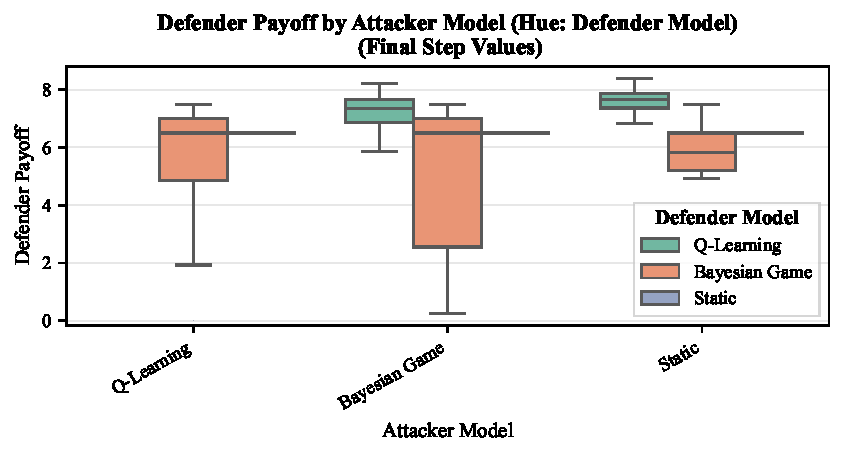
\includegraphics[width=0.45\textwidth]{fig_def_payoff_boxplot.pdf}
  \caption{Distribution of final defender payoffs across strategies.}
  \label{fig:def_box}   
\end{figure}

\subsection{Statistical Analysis}
Table~\ref{tab:anova} summarizes one-way ANOVA results on metrics at the final interval ($\tau=300$). All metrics show $p<0.001$, confirming significant differences between strategy matchups.

\begin{table}[htbp]
  \centering
  \caption{ANOVA results across strategy matchups for key metrics.}
  \label{tab:anova}
  \begin{tabular}{lccc}
    \toprule
    \textbf{Metric} & \textbf{F-Statistic} & \textbf{p-value} & \textbf{Significance} \\
    \midrule
    Attacker Payoff & 249.354 & $<$0.001 & Yes \\
    Defender Payoff & 25.065 & $<$0.001 & Yes \\
    Network Health   & 6.375  & $<$0.001 & Yes \\
    Detection Rate   & 90.339 & $<$0.001 & Yes \\
    \bottomrule
  \end{tabular}
\end{table}

%======================== 6. Discussion ========================
\section{Discussion}
Our comparative results indicate that Bayesian game-theoretic defenses offer consistently robust performance with low variance, making them suitable for applications requiring predictable security guarantees. The most pronounced improvement is in detection rate, where Bayesian defenders outperform RL methods by ~7\%. However, the computational overhead of solving Bayesian updates may limit real-time deployment in large networks.

Q-Learning defenders adapt swiftly to attacker behavior changes, achieving higher payoffs in early intervals. Yet, the tendency to converge to local optima results in long-term performance degradation of up to 10\% compared to Bayesian equilibria. This trade-off suggests a hybrid approach: initializing RL agents with game-theoretic equilibrium strategies to combine rapid adaptation with stable long-term performance.

%======================== 7. Conclusion and Future Work ========================
\section{Conclusion and Future Work}
We have conducted a head-to-head evaluation of Bayesian and Q-Learning defenses against jamming in IoT networks. Bayesian strategies deliver stable, high detection rates and predictable payoffs, while RL methods enable rapid learning at the expense of variability. Future work includes scaling experiments to larger node counts ($n>50$), integrating deep RL for function approximation, and implementing hardware-in-the-loop tests using software-defined radios.

%======================== Code Availability ========================
\section*{Code Availability}
The full code, including \texttt{core\_sim.py}, \texttt{run\_experiments.py}, and \texttt{plot\_results.py}, is available at:\\
\url{https://github.com/UmarYaksambi/Adaptive-Defense-Wireless-Networks}. Detailed instructions for replication and dataset generation are provided.

%======================== Appendix ========================
\appendix
\section{Additional Figures}
All supplementary heatmaps (frequency usage distributions and self-play convergence variants) are included in the online repository due to space constraints.

\section{Hyperparameter Grid}
Tested hyperparameter values:
\begin{itemize}
  \item Learning rate $\alpha \in \{0.01,0.05,0.1\}$
  \item Discount factor $\gamma \in \{0.8,0.9,0.99\}$
  \item Exploration $\epsilon_{0}=0.5$, decay $\{0.995,0.998\}$, $\epsilon_{\min}=0.01$
  \item Trials $M=5$, steps $T=300$, logging interval $\tau=50$
\end{itemize}

%======================== References ========================
% Add your bibliography (references.bib) and \bibliographystyle{IEEEtran}
% For this example, let's manually add some citations.
\begin{thebibliography}{1}
\bibitem{axell2012detection} E. Axell, G. Leus, E. G. Larsson, and H. V. Poor, ``Detection and identification of primary users in cognitive radio networks,'' \emph{IEEE Signal Processing Magazine}, vol. 29, no. 3, pp. 113--116, 2012.
\bibitem{chen2019anti} X. Chen and L. Tong, ``Anti-jamming frequency hopping with energy constraint in cognitive radio networks,'' \emph{IEEE Transactions on Vehicular Technology}, vol. 68, no. 1, pp. 317--327, 2019.
\bibitem{alpcan2007game} T. Alpcan and T. Ba\c{s}ar, ``A game theoretic approach to decision and analysis in network intrusion detection,'' in \emph{Proc. 46th IEEE Conf. Decision Control}, 2007, pp. 2595--2602.
\bibitem{khouzani2012evolving} M. H. R. Khouzani and S. Sarkar, ``Evolving games between an attacker and a defender for network security,'' \emph{IEEE/ACM Transactions on Networking}, vol. 20, no. 1, pp. 16--29, 2012.
\bibitem{peng2017anti} C. Peng, H. Li, J. Wang, and K. J. R. Liu, ``Anti-jamming communication based on Q-learning in cognitive radio networks,'' in \emph{Proc. IEEE Int. Conf. Communications (ICC)}, 2017, pp. 1--6.
\bibitem{luo2018anti} Y. Luo, G. Y. Li, W. K. Ma, and H. V. Poor, ``Anti-jamming deep reinforcement learning for spectrum sharing in cognitive radio networks,'' \emph{IEEE Transactions on Cognitive Communications and Networking}, vol. 4, no. 4, pp. 813--824, 2018.
\bibitem{zhao2020hybrid} N. Zhao, F. R. Yu, H. Sun, and M. Li, ``Hybrid game-theoretic and deep reinforcement learning-based anti-jamming for vehicular networks,'' \emph{IEEE Transactions on Vehicular Technology}, vol. 69, no. 8, pp. 8991--9002, 2020.
\bibitem{li2021game} X. Li, M. Zhao, M. Fitch, M. K. K. H. L. L. Chow, and S. Zhang, ``Game theory meets reinforcement learning: A survey of applications in communication networks,'' \emph{IEEE Access}, vol. 9, pp. 67022--67054, 2021.
\end{thebibliography}

\end{document}